% !TeX spellcheck = es_ES
\documentclass{scrartcl}
%\documentclass{book}
\usepackage[spanish]{babel}
\usepackage[utf8]{inputenc}
\usepackage{enumerate}
\usepackage{graphicx}
\usepackage{color}
\usepackage{float}
\usepackage{multicol}
\usepackage{listings}%codigo de programación
\usepackage{lscape}
\usepackage{fancyhdr}
\usepackage{tabularx}
\usepackage[hidelinks,colorlinks=true, linkcolor=black]{hyperref} %hyperref para hacer los links del indice y usar \url{URL} y \href{URL}{text}y hidelinks para que no se rodeen con una caja de color los enlaces. Más información en: http://en.wikibooks.org/wiki/LaTeX/Hyperlinks




\pagestyle{fancy}
%\usepackage{tabulary}
%\usepackage{/home/manolito/IISSI/pruebaLaTex/comfortaa/tex/latex/comfortaa/comfortaa}

\lfoot[\thepage]{\bfseries{
\includegraphics[width=0.020\textwidth]{imagenes/logo.png} PhotoLoad}}
\cfoot[\thepage]{}
\rfoot[\thepage]{\thepage}
%\lfoot[c1]{GECH}
%\lfoot[e1]{GECH}
\lhead[\thepage]{}
\rhead[\thepage]{}
\renewcommand{\headrulewidth}{0.0pt}
\renewcommand{\footrulewidth}{0.2pt}
\hyphenation{se-ma-nal per-so-na-les ope-ra-tivo mo-ni-tor mues-tra pide correc-ta-men-te}



%\renewcommand{\baselinestretch}{1.5} %interlineado

\begin{document}
%\begin{figure}[H]
%	\centering
%	\makebox[\textwidth]{\includegraphics[width=0.98\textwidth]{/home/manolito/datos/IISSI/Portada/V2.png}}
%	%\caption{BPMN1}
%	\label{fig:Portada}
%\end{figure}
%\thispagestyle{empty}
%\pretolerance=2000
%\tolerance=3000
\begin{titlepage}
\begin{center}
	\vspace*{-1in}
%	\begin{figure}[htb]
%		\begin{center}
%			
\includegraphics[width=8cm]{./figuras/logo}
%		\end{center}
%	\end{figure}
	\vspace*{2in}
	\begin{Huge}
		%si lo quieres poner mas grande Huge, huge, uno mas pequeño LARGE, dos más pequeños Large
		\textbf{PhotoLoad} \\
	\end{Huge}
	\vspace*{0.15in}	
	\begin{LARGE}
		\textsc{Publica y descarga las fotos de cada día}
	\end{LARGE}\\
	\vspace*{0.2in}	
	\begin{figure}[H]
		\centering
		\makebox[\textwidth]{
\includegraphics[width=0.3\textwidth]{imagenes/logo.png}}
		%\caption{Interfaz de descarga}
		\label{fig:logo}
	\end{figure}Desplegada en: \href{https://etsiiphotoload.appspot.com}{https://etsiiphotoload.appspot.com}\\Código fuente: \href{https://github.com/ManuelLR/PhotoLoad}{https://github.com/ManuelLR/PhotoLoad}
	\vspace*{0.1in}
	\rule{140mm}{0.1mm}\\
	\vspace*{0.1in}
	\begin{Large}
	Arquitectura e Integración de Sistemas Software\\	
	Segundo Curso del Grado de Ingeniería del Software\\
	Grupo 2\\
	Universidad de Sevilla\\	

	\end{Large}\\
	\vspace*{0.4in}
	\underline{Realizado por:} \\
		\vspace*{0.1in}
		\begin{large}
		Manuel Francisco López Ruiz (\href{mailto:manloprui1@alum.us.es}{manloprui1@alum.us.es})\\
		Miguel Rodríguez Caballero (\href{mailto:miguel.rc95@gmail.com}{miguel.rc95@gmail.com})\\
		David Tinoco Castillo (\href{mailto:daviid.tc@gmail.com}{daviid.tc@gmail.com})\\ 
		\end{large}
	%\rule{70mm}{0.1mm}\\
		\vspace*{0.2in}
		\underline{Tutorizado por:}\\
		\vspace*{0.1in}
		Ana Belén Sánchez Jerez (\href{mailto:anabsanchez@us.es}{anabsanchez@us.es})\\

	
%	\vspace*{0.6in}
	
\end{center}
\end{titlepage}
\newpage

\tableofcontents % indice de contenidos
\newpage

\section{Introducción}
Hoy en día subir fotos a las redes sociales es una tarea tediosa y descargarlas es más complicado aun pero, si además queremos hacer esto con todas las fotos a la vez, ya se convierte en algo imposible.

Es ahí donde interviene PhotoLoad, un sencillo mashup ideado para facilitar estas tareas que todos realizamos alguna vez. Tras iniciar sesión mediante PhotoLoad en las aplicaciones que desees usar, podrás ver las fotos de todos tus dispositivos pudiendo publicarlas en Facebook o Flickr con un solo click. Pero la mayor funcionalidad de PhotoLoad radica de la posibilidad de descargar las fotos de Facebook y Flickr en Google Drive, Dropbox o a tu ordenador con un simple click, ya sean pocas o muchas, con PhotoLoad podrás hacerlo. 


%PhotoLoad es un mashup destinado a todos aquellos que tienen perfiles en redes sociales. Con él podrás publicar facilmente tus fotos en Facebook o Instagram. Además, podrás guardar las fotos de Facebook e Instagram en  de poder guardar las fotos que quieres a funcionalidad más interesante de este mashup reside en el 

%Aprovechando que, actualmente, la mayoria de fotos se toman con el móvil y un alto porcentaje poseen la aplicación Google Fotos la cual por defecto sube las fotos a la nube de Google (sin publicarlas), sería posible crear un mashups que te permitiera ver esas fotos que se suben automáticamente con la opción de publicarlas en aplicaciones sociales como Facebook e Instagram. Puesto que no todo el mundo necesita hacer este proceso, el cual se puede hacer directamente desde las aplicaciones nativas, planteamos que esta aplicación, a su vez, pudiera hacer el proceso inverso, es decir, que permita guardar todas las fotos de Facebook e Instagram en Google Fotos o descargarlas para así conservar todos los recuerdos que caen en el olvido en las redes sociales. 

\subsection{Aplicaciones Integradas}\label{cap:APIs Integradas}
Como se ha mencionado anteriormente, PhotoLoad integrará 4 aplicaciones:
\begin{enumerate}[\textbf{\textperiodcentered}]
	\item \textbf{Facebook} (\url{https://developers.facebook.com/docs/javascript}). API de la cual se pueden publicar fotos en el muro y descargar fotos. Esta aplicación se ha implementado mediante OAuth2 y servicio Rest.
	\item \textbf{Flickr} (\url{https://www.flickr.com/services/api/}). API de la cual se pueden descargar fotos. Esta aplicación mediante OAuth1 y servicio Rest.
	\item \textbf{Google Drive} (\url{https://developers.google.com/drive/}), la cual integra la anteriormente denominada Picasa Web Album. De esta API se obtienen las fotos de los dispositivos gracias a la aplicación Android denominada "Fotos" la cual realiza copias de seguridad de ellas automáticamente. Esta API nos permitirá descargar fotos (de la copia de seguridad y de otras fuentes). Esta aplicación se ha implementado mediante OAuth2 y servicio Rest.
	\item \textbf{Dropbox} (\url{https://www.dropbox.com/developers/core}). De esta API se pueden exportar las fotos para publicarlas en las redes sociales o importarlas de las mismas. Esta aplicación se ha implementado mediante OAuth2 y servicio Rest.
	
\end{enumerate}
\subsection{Evolución del proyecto}\label{cap:problemas encontrados}
\subsubsection{Integración con Google Drive}
Durante la exploración de la api de Google Fotos, vimos que habían realizado un cambio en el funcionamiento de la misma, lo que no nos permitía usarla como teníamos planeado. Por ello decidimos sustituirla por Google Drive en la cual podías incluir una carpeta con tus fotos de Google Fotos mediante una nueva función fruto del cambio de la api por parte de Google. En este punto nos encontramos con la dificultad, que aún no hemos subsanado, de navegar entre las carpetas de Google Drive lo que nos imposibilita acceder directamente a la carpeta de fotos para evitar molestias al usuario final de la aplicación. A su vez, hemos conseguido descargar los archivos al ordenador pero no ha sido posible obtener el enlace de descarga de los mismos para poder subirlos directamente a los otros servicios que integra PhotoLoad.

Aparte de dichos problemas, también se han encontrado los problemas comunes detallados en el apartado \ref{cap:problemasComunesEncontrados}.
\subsubsection{Integración con Dropbox}
Inicialmente, Dropbox se iba a usar mediante dos apis: \href{https://www.dropbox.com/developers/dropins/chooser/js}{Dropbox Chooser} y \href{https://www.dropbox.com/developers/dropins/saver}{Dropbox Saver}. Estas apis se decidieron sustituir por los servicios Rest prestados mediante la \href{https://www.dropbox.com/developers/core}{Dropbox Core API} (\href{https://www.dropbox.com/developers/core/docs}{Rest}) ya que, las otras apis, estaban preparadas para integrarlas directamente en una web impidiéndonos pasar los archivos entre los diferentes servicios sin descargarlos en el ordenador. Tras el cambio de aplicación, primero nos encontramos problemas con la autenticación debido a que Dropbox solo permite el envío y reenvío de peticiones mediante conexión cifrada (https), y después tuvimos algún que otro problema relacionado con los permisos asignados a la aplicación desde Dropbox.

La subida de archivos no se ha podido implementar hasta la fecha debido a la mala documentación por parte de Dropbox.

Aparte de dichos problemas, también se han encontrado los problemas comunes detallados en el apartado \ref{cap:problemasComunesEncontrados}.

\subsubsection{Integración con Facebook}
Esta api fue la última api que implementamos ya que, esperamos hasta realizar la práctica en la que se realizarían peticiones a Facebook mediante OAuth2 (práctica 7). Aun así, nos encontramos con el problema de que no se podían hacer peticiones que implicarán datos del usuario, a pesar de tener el acces\_token (ni en la misma práctica se pudieron realizar). Esto se debía al reciente cambio de políticas en los permisos para realizar las peticiones que había implementado Facebook (justamente la noche anterior a la realización de la práctica 7). Tras esto, decidimos pedir a Facebook los permisos necesarios, los cuales fueron rechazados dos veces (estamos esperando la respuesta de la tercera petición). Para solventar este problema, añadimos una caja de texto la cual se rellena automáticamente con el access\_token pero que, debido a los permisos ofrecidos a nuestra aplicación por parte de Facebook, no es válido para realizar las peticiones. En su lugar se puede generar un access\_token desde este link: \url{https://developers.facebook.com/tools/explorer/}. Necesitaremos seleccionar (mediante el botón Get Token) los permisos de user\_photos (para obtener tus fotos) y, en la sección Extended Permission de esa misma ventana emergente, seleccionaremos publish\_actions (para poder publicar las fotos). Tras esto, solo deberemos sustituir el access\_token  proporcionado por PhotoLoad por el obtenido desde Facebook manualmente.

La aplicación y los servicios Rest no dieron ningún tipo de problemas.

\subsubsection{Integración con Flickr}
Esta api ha sido la más complicada y problemática desde el inicio del proyecto. Primeramente se iba a usar Instagram, a pesar de que no dispusiera de librerías en java pero, al comprobar que solo se permitía la subida de fotos desde sus aplicaciones oficiales \footnote{Véanse las últimas líneas de la documentación oficial: \url{https://instagram.com/developer/endpoints/media/}}, decidimos reemplazarla por Flickr, la cual se parece a Intragram pero orientada a un ámbito más serio y profesional.

Flickr no mantiene ninguna librería para interactuar con la aplicación si no que muestra una lista de las librerías creadas por los usuarios. Debido a esta característica decidimos implementarlo como servicio Rest ya que de esta manera nos aseguraríamos el correcto funcionamiento. Además de todo esto, Flickr usa OAuth1 para la autenticación de los usuarios, lo que supuso un gran esfuerzo por el grupo para conseguir la integración y el login. En primer lugar buscamos algunas librerías y decidimos implementar la  \href{http://oauth.googlecode.com/svn/code/java/core/}{librería de oauth} distribuida desde su página web oficial (\url{oauth.net}). Tras varios días intentando entenderla, implementarla y usarla, decidimos dejarla ya que no habíamos conseguido ningún tipo de avance. Posteriormente, decidimos volver a la web oficial y encontramos otra librería denominada \href{https://github.com/mttkay/signpost}{OAuth-Signpost}. Esta librería fue más complicada todavía ya que tuvimos que aprender a compilar con Maven desde terminal, instalando todos los complementos que requería para ser utilizada. Tras compilarla, encontrar errores de código, corregirlos y recompilar múltiples veces lo único que conseguimos tras tres días fue el mecanismo para firmar las peticiones. Una de las mayores dificultades de esta librería, era la gran modularidad que tenía, llegando a ser tal que no se sabía de que modulo se debían usar las clases. 

Tras varios días de búsqueda, encontramos la librería denominada \href{https://github.com/fernandezpablo85/scribe-java}{Scribe}. Tras compilarla, en media tarde pudimos hacer un login a Flickr desde la terminal, consiguiendo el access\_token y todo lo necesario para hacer la primera petición de prueba. Ahora debíamos implementarlo para que funcionara como aplicación GWT con todo lo que ello conlleva ya que, todos los login debían estar en la parte de servidor y solo se le debía dar al cliente los datos necesarios. Tras varios días, conseguimos implementarlo aunque unos días después tuvimos que hacerlo desde el principio ya que, los datos de la autenticación se guardaban en el servidor por lo que no era posible que mas de un usuario pudiera usar la aplicación al mismo tiempo. Tras las modificaciones oportunas, la creación de clases y los parches necesarios para usar esas clases con \href{https://github.com/fernandezpablo85/scribe-java}{Scribe}, conseguimos un login funcional en GWT desde la interfaz gráfica.

Posteriormente nos encontramos con el problema que conlleva la realización de peticiones mediante el método de OAuth1, la cual debe llevar una firma que sirve para comprobar que los datos hayan llegado correctamente. Por suerte no hubo problema en este apartado, pero no se puede decir lo mismo del parseo de los datos recibidos por las peticiones. La librería \href{https://github.com/fernandezpablo85/scribe-java}{Scribe} incluye los objetos JSONObject, los cuales sirven para parsear los datos pero, tras entender su funcionamiento, tuvimos que crear las clases de los objetos manualmente y, después de descubrir que Flickr añade a sus respuestas atributos que impiden el parseo por parte de JSONObject, conseguimos hacer funcionar satisfactoriamente las peticiones en una aplicación java local. Al adaptarlo para GWT aparecieron errores, antes inexistentes, debido a problemas con la librería JSONObject por lo que nos vimos en la obligación de usar otras incluidas ya en GWT.

Tras todos estos problemas con Flickr, conseguimos implementar las visualización de las fotos en nuestra aplicación sin mayores problemas. La subida de fotos no se ha podido implementar todavía debido al tiempo consumido por esta api.

Aparte de dichos problemas, también se han encontrado los problemas comunes detallados en el apartado \ref{cap:problemasComunesEncontrados}.

\subsubsection{Problemas comunes encontrados}\label{cap:problemasComunesEncontrados}
Contar el problema de la descarga de archivos eeeeeeeeeeeeeeeeeeeeeeeeeeeeeeeeeeeeeeeeeeeeee
eeeeeeeeeeeeeeeeeeeeeeeeeeeeeeeeeeeeeeeeeeeee
eeeeeeeeeeeeeeeeeeeeeeeeeeeeeeeeeeeeeeeeeeeee
eeeeeeeeeeeeeeeeeeeeeeeeeeeeeeeeeeeeeeeeeeeee
eeeeeeeeeeeeeeeeeeeeeeeeeeeeeeeeeeeeeeeeeeeee
eeeeeeeeeeeeeeeeeeeeeeeeeeeeeeeeeeeeeeeeeeeee
eeeeeeeeeeeeeeeeeeeeeeeeeeeeeeeeeeeeeeeeeeeee
eeeeeeeeeeeeeeeeeeeeeeeeeeeeeeeeeeeeeeeeeeeee
eeeeeeeeeeeeeeeeeeeeeeeeeeeeeeeeeeeeeeeeeeeee
eeeeeeeeeeeeeeeeeeeeeeeeeeeeeeeeeeeeeeeeeeeee
eeeeeeeeeeeeeeeeeeeeeeeeeeeeeeeeeeeeeeeeeeeee
eeeeeeeeeeeeeeeeeeeeeeeeeeeeeeeeeeeeeeeeeeeee
eeeeeeeeeeeeeeeeeeeeeeeeeeeeeeeeeeeeeeeeeeeee
eeeeeeeeeeeeeeeeeeeeeeeeeeeeeeeeeeeeeeeeeeeee
eeeeeeeeeeeeeeeeeeeeeeeeeeeeeeeeeeeeeeeeeeeee
eeeeeeeeeeeeeeeeeeeeeeeeeeeeeeeeeeeeeeeeeeeee
eeeeeeeeeeeeeeeeeeeeeeeeeeeeeeeeeeeeeeeeeeeee
eeeeeeeeeeeeeeeeeeeeeeeeeeeeeeeeeeeeeeeeeeeee
eeeeeeeeeeeeeeeee
\section{Prototipos de Interfaz de Usuario}\label{cap:prototipos interfaz}
A continuación se definirán los prototipos de interfaz (mockup) de PhotoLoad. Se explicará cada vista por separado acompañada de un boceto. La iteración entre vistas se detallará en la sección \ref{cap:DiagramaVistas} (página \pageref{cap:DiagramaVistas}).
% es un mashup con interfaz web por lo que debe quí podemos ver una demo(no se como llamarle xd) de como sera la interfaz gráfica de nuestro mashap
\subsection{Interfaz de inicio}\label{cap:InterfazInicio}
Esta vista (Figura \ref{fig:VistaLogin}) será la primera que vea el usuario al acceder a la aplicación. En ella el usuario podrá elegir si desea usar la aplicación o ir a la página de información.

\begin{figure}[H]
	
	\centering
	\makebox[\textwidth]{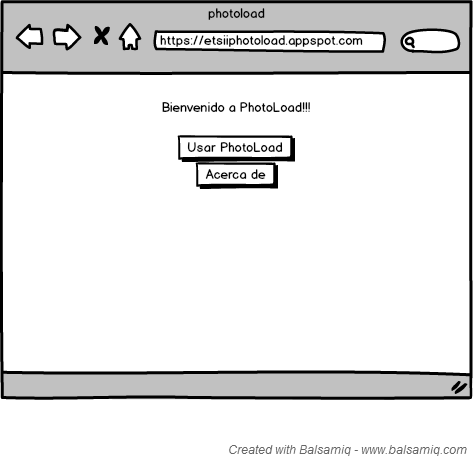
\includegraphics[width=0.8\textwidth]{imagenes/vistaLogueo.png}}
	\caption{Interfaz de inicio}
	\label{fig:VistaLogin}
	
\end{figure}

%\vspace*{2in}
\subsection{Interfaz de selección de descarga}
Esta vista (Figura \ref{fig:VistaSubida}) permitirá al usuario seleccionar desde que aplicación desea descargar las fotos que posteriormente subirá. A su vez podrá ir a la página de Inicio (sección \ref{cap:InterfazInicio}).
%Si al loguearte seleccionaste subir fotos, llegaras hasta aquí, donde puedes elegir desde donde quieres subir tus fotos (google fotos, dropbox o tu pc), hasta a que red social subirla una vez que hayas elegido las fotos!
\begin{figure}[H]
	
	\centering
	\makebox[\textwidth]{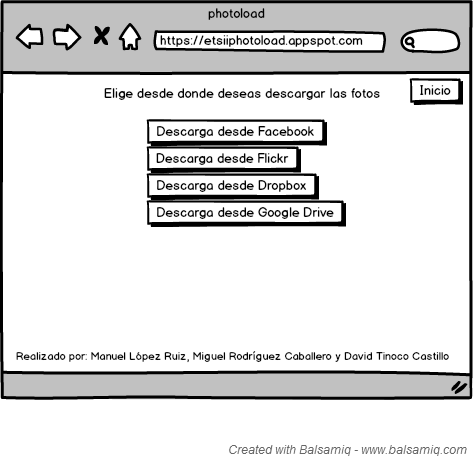
\includegraphics[width=0.8\textwidth]{imagenes/processView.png}}
	\caption{Interfaz de selección de descarga}
	\label{fig:VistaSubida}
	
\end{figure}
\subsection{Interfaz de cada aplicación}
Esta vista dependerá de cada aplicación aunque podremos diferenciar claramente entre la de descarga (Ejemplo: Figura \ref{fig:VistaDescargaDropbox}) y la de publicación (Ejemplo: Figura \ref{fig:VistaSubidaFacebook}).

%Si al loguearte seleccionaste subir fotos, llegaras hasta aquí, donde puedes elegir desde donde quieres subir tus fotos (google fotos, dropbox o tu pc), hasta a que red social subirla una vez que hayas elegido las fotos!
\begin{figure}[H]
	
	\centering
	\makebox[\textwidth]{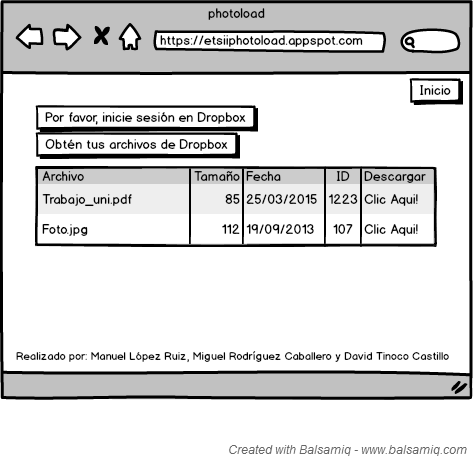
\includegraphics[width=0.8\textwidth]{imagenes/descargaDe.png}}
	\caption{Interfaz de descarga de Dropbox}
	\label{fig:VistaDescargaDropbox}
	
\end{figure}
\begin{figure}[H]
	
	\centering
	\makebox[\textwidth]{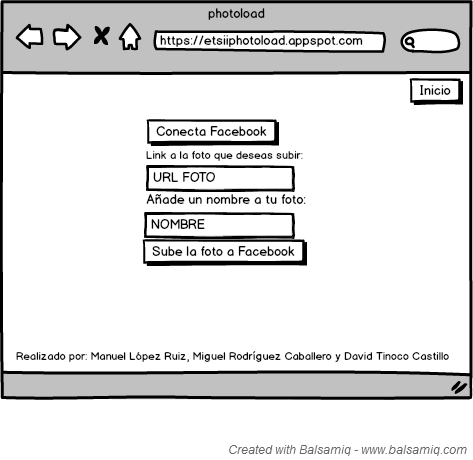
\includegraphics[width=0.8\textwidth]{imagenes/subeA.png}}
	\caption{Interfaz de subida de Facebook}
	\label{fig:VistaSubidaFacebook}
	
\end{figure}
%\vspace*{2in}
\subsection{Interfaz de selección de publicación}
Esta vista (Figura \ref{fig:VistaDescarga}) permitirá al usuario seleccionar a donde desea subir las fotos.

%Si al loguearte seleccionaste bajar fotos, llegaras hasta esta otra vista, donde deberás elegir que fotos descargar hacia tu dropbox!
\begin{figure}[H]
	
	\centering
	\makebox[\textwidth]{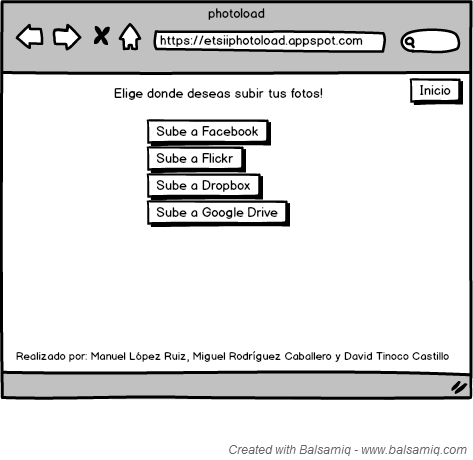
\includegraphics[width=0.8\textwidth]{imagenes/publishView.png}}
	\caption{Interfaz de descarga}
	\label{fig:VistaDescarga}
	
\end{figure}
%\vspace*{2in}
\section{Arquitectura}

\subsection{Diagrama de Componentes}
El diagrama de componentes (Figura \ref{fig:DiagramaComponentes}) muestra las aplicaciones usadas en el mockup y como enlazarán con PhotoLoad. Se nutre de un total de 4 APIs.

\begin{figure}[H]
	
	\centering
	\makebox[\textwidth]{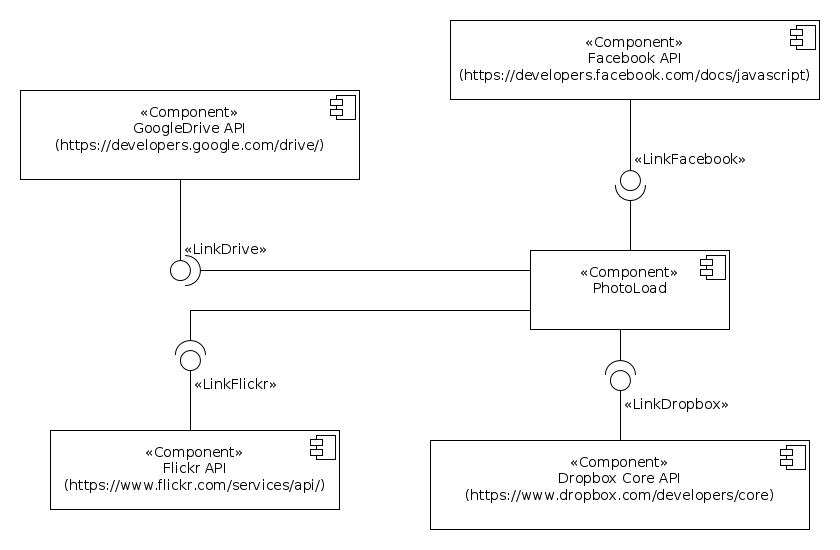
\includegraphics[width=1\textwidth]{imagenes/umlComponentesPhotoLoad.png}}
	\caption{Diagrama de Componentes}
	\label{fig:DiagramaComponentes}
	
\end{figure}

\subsection{Diagrama de Despliegue}
El diagrama de despliegue (Figura \ref{fig:DiagramaDespliegue}) muestra como se desplegará PhotoLoad en el servidor (AppEngine) y como lo hará en el navegador web del cliente.

\begin{figure}[H]
	
	\centering
	\makebox[\textwidth]{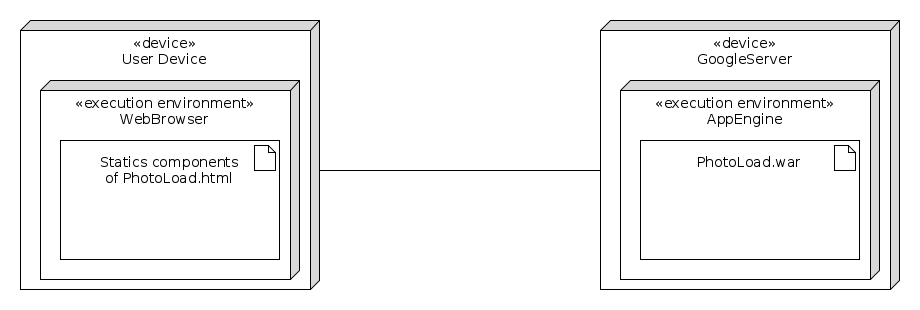
\includegraphics[width=1\textwidth]{imagenes/umlDesplieguePhotoLoad.png}}
	\caption{Diagrama de Despliegue}
	\label{fig:DiagramaDespliegue}
	
\end{figure}
\subsection{Diagrama de Vistas}\label{cap:DiagramaVistas}
El diagrama de vistas (Figura \ref{fig:DiagramaVistas}) muestra como se podrá ir navegando por las diferentes vistas de PhotoLoad.
\begin{figure}[H]
	
	\centering
	\makebox[\textwidth]{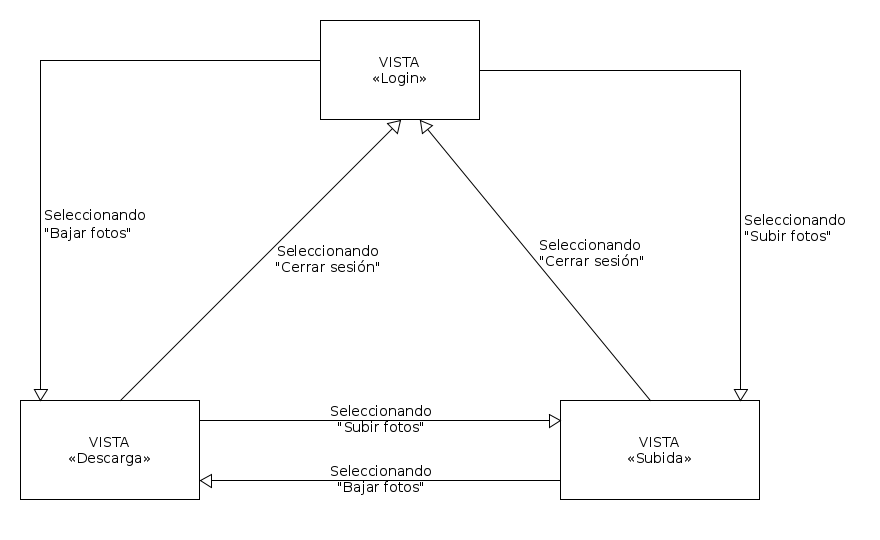
\includegraphics[width=1\textwidth]{imagenes/umlDiagramaVistas.png}}
	\caption{Diagrama de Vistas}
	\label{fig:DiagramaVistas}
	
\end{figure}
\subsection{Diagrama de Clases}
En esta fase del proyecto no está suficientemente definido el diagrama de clases por lo que se pondrá en futuros entregables.
\section{Pruebas}\label{cap:pruebas}
A continuación se expondrá la estructura de las pruebas realizadas en JUnit y separadas por Apis.
\subsection{Facebook}

\begin{tabularx}{14cm}{|c|X|}
	\hline \textbf{ID} & Prueba FB1\\ 
	\hline \textbf{Descripción} & Comprueba la correcta obtención de las fotos existentes en Facebook para el usuario \\	 
	\hline  \textbf{Entrada}		& Token \\ 
	\hline  \textbf{Salida esperada}			& Lista de Fotos\\
	\hline  \textbf{Resultado}			& Exito \\
	\hline 
	\end{tabularx} 
\\
\\

\begin{tabularx}{14cm}{|c|X|}
		\hline \textbf{ID} & Prueba FB2\\ 
		\hline \textbf{Descripción} & Comprueba la correcta subida de fotos al tablon de Facebook \\	 
		\hline  \textbf{Entrada}		& Token y url de la foto a subir \\ 
		\hline  \textbf{Salida esperada}			& El id de la foto subida\\
		\hline  \textbf{Resultado}			& Exito \\
		\hline 
		\end{tabularx} 
\subsection{Flickr}

\begin{tabularx}{14cm}{|c|X|}
	\hline \textbf{ID} & Prueba FL1 \\ 
	\hline \textbf{Descripción} & Comprueba el correcto funcionamiento de las dos fases de login necesarios para Flickr \\	 
	\hline  \textbf{Entrada}		& No entra ningún dato \\ 
	\hline  \textbf{Salida esperada}			& Un objeto de tipo OAuth con una URL y un AccessToken relleno\\
	\hline  \textbf{Resultado}			& Exito \\
	\hline 
\end{tabularx} 
\\
\\

\begin{tabularx}{14cm}{|c|X|}
	\hline \textbf{ID} & Prueba FL2 \\ 
	\hline \textbf{Descripción} & Comprueba la correcta obtención de las fotos existentes en Flickr para el usuario \\	 
	\hline  \textbf{Entrada}		& Token (OAuth) \\ 
	\hline  \textbf{Salida esperada}			& Lista de FlickrPhoto no null con los ids de las fotos pero sin los links de descarga\\
	\hline  \textbf{Resultado}			& Exito \\
	\hline 
\end{tabularx} 
\\
\\

\begin{tabularx}{14cm}{|c|X|}
	\hline \textbf{ID} & Prueba FL3\\ 
	\hline \textbf{Descripción} & Comprueba la correcta obtención de los links de las fotos existentes en Flickr para el usuario \\	 
	\hline  \textbf{Entrada}		& Token (OAuth) y lista de FlickrPhoto de las que queremos obtener el link \\ 
	\hline  \textbf{Salida esperada}			& Lista de FlickrPhoto con la información anterior además de links de descarga\\
	\hline  \textbf{Resultado}			& Exito \\
	\hline 
\end{tabularx} 
\subsection{Dropbox}
Estas pruebas son muy sencillas, ya que consisten en ver que los métodos implementados son capaces de obtener archivos (testGetAll), crear archivos en Dropbox (testInsert) y descargarlos (testDownload).

\subsubsection{Test GetAll}
El primero de ellos consiste en hacer una llamada al método getFolder, el cual nos dará la información de los archivos y las carpetas que pertenezcan a la ruta que les pasamos como id (vacía en este caso). Después lo que hacemos es comprobar que el archivo resultante no es nulo, y mostraremos todas las carpetas y documentos que guarda mediante un bucle for.

\subsubsection{Test Insert}
En este test lo que hacemos es lo siguiente. Primero, creamos un archivo el cual queremos subir a Dropbox, después le indicamos la ruta en la que se debe crear y con que nombre (en la ruta id con el nombre Fichero\_a\_insertar). Una vez creado el archivo, creamos una cadena de texto el cual será el contenido de ese archivo que vamos a subir y hacemos una llamada al método insertFile pasándole como parámetros la ruta, el archivo a subir y su contenido. Finalmente, comprovamos que el fichero no es nulo y mostramos por pantalla el id y la ruta del archivo.

\subsubsection{TestDownload}
Sin duda es el test mas simple de todos. Llamamos al método downloadFile y le pasamos la ruta del archivo a descargar. Este método devuelte una cadena de texto, la cual es la url del archivo. Comprobamos que la cadena de texto no es nula y la mostramos por pantalla.

\subsection{Google Drive}
\begin{tabularx}{14cm}{|c|X|}
	\hline \textbf{ID} & Prueba GD1 \\ 
	\hline \textbf{Descripción} & Comprueba el correcto funcionamiento al solicitar la lista de archivos a la cuenta de Google Drive logeada. \\	 
	\hline  \textbf{Entrada}		& Token (OAuth) \\ 
	\hline  \textbf{Salida esperada}			& Lista de archivos del Google Drive del usuario \\
	\hline  \textbf{Resultado}			& Éxito	 \\
	\hline 
\end{tabularx} 
\\
\\

\begin{tabularx}{14cm}{|c|X|}
	\hline \textbf{ID} & Prueba GD2 \\ 
	\hline \textbf{Descripción} & Comprueba el correcto funcionamiento al intentar descargar un archivo de la cuenta de Google Drive logeada.\\	 
	\hline  \textbf{Entrada}		& Token(OAuth) e índice del archivo a descargar en la lista \\ 
	\hline  \textbf{Salida esperada}			& URL para descargar dicho archivo \\
	\hline  \textbf{Resultado}			& Éxito \\
	\hline 
\end{tabularx} 
\section{Api Rest}\label{cap:apiRest}
PhotoLoad también integra una Api Rest para que los usuarios más experimentados puedan intercambiar comentarios entre ellos. Dicha api esta alojada en la siguiente url: \href{https://etsiiphotoload.appspot.com/api}{https://etsiiphotoload.appspot.com/api}. 

Las peticiones que se podrán realizar a la api vienen recogidas en la siguiente tabla:
\\

\begin{tabularx}{14cm}{|c|X|X|}
	\hline \textbf{HTTP} & \textbf{Plantilla URI} &\textbf{Descripción}\\ 
	\hline GET & /comments & Obtiene una lista con todos los comentarios.\\	 
	\hline  GET		& /comments/\{index\}& Obtiene el comentario con dicho índice.\\ 
	\hline  POST			& /comments & Añade un nuevo comentario.
	Si se añade correctamente devuelve un mensaje “201 Uploaded”.
	Si ocurre algún error devuelve “400 Error”.\\
	\hline  PUT			& /comments/edit/\{index\}	& Sustituye el comentario con dicho índice por el que indiques.
	Si se realiza correctamente, debe devolver un “204 No Content”. Si el comentario, debe devolver un “404 Not Found”.\\
	\hline  DELETE			& /comments/delete/\{index\}	& Borra el comentario con dicho índice.
	Si se realiza correctamente, debe devolver un “204 No Content”. Si el comentario no existe debe devolver un “404 Not Found”.\\
	\hline 
\end{tabularx} 
\newpage
Ahora pondremos algunos ejemplos de respuestas en formato JSON (el cual ofrece nuestra API):
\\

GET: \href{https://etsiiphotoload.appspot.com/api/comments}{https://etsiiphotoload.appspot.com/api/comments}

\begin{lstlisting}[frame=lrtb,numbers=left]
-0: {
	contenido: "Que gran aplicacion!"
}
-1: {
	contenido: "¿Por que no quedamos el sabado?"
}

\end{lstlisting}
%\hline

\\
GET: \href{https://etsiiphotoload.appspot.com/api/comments/0}{https://etsiiphotoload.appspot.com/api/comments\{id\}}

\begin{lstlisting}[frame=lrtb,numbers=left]
{
contenido: "Que gran aplicacion!"
}
\end{lstlisting}

\section{Historial de Versiones}
Este apartado muestra el historial de versiones mediante la siguiente tabla:
\\

\begin{tabularx}{14.9cm}{|c|c|X|X|}
	\hline \textbf{Fecha} & \textbf{Versión} & \centering \textbf{Detalles} & \textbf{Participantes} \\ 
	\hline 22-03-2015 & 1.0 & Incluye introducción, prototipos de las interfaces de usuario y diagramas UML de componentes y despliegue.  & 
	López Ruiz, Manuel Francisco
	
	Rodríguez Caballero, Miguel
	
	Tinoco Castillo, David \\	 
		\hline 10-05-2015 & 2.0 & \begin{enumerate}[\textbf{\textperiodcentered}]
		\item \textbf{Mejora de la versión 1.0}: Cambios en la Figura \ref{fig:DiagramaDespliegue} y otros cambios menores. 
		 \item \textbf{Cambio de APIs} reflejado en el apartado \ref{cap:APIs Integradas} y todos los cambios que conlleva respecto al entregable anterior. También se ha explicado el tipo de servicio usado con cada api.
		
		\item \textbf{Ampliación} del apartado \ref{cap:herramientas} y del apartado \ref{cap:problemas encontrados} con los problemas encontrados en esta entrega  . \end{enumerate}
		 & 
		López Ruiz, Manuel Francisco
		
		Rodríguez Caballero, Miguel
		
		Tinoco Castillo, David \\
		\hline 31-05-2015 & 3.0 & \begin{enumerate}[\textbf{\textperiodcentered}]
			\item \textbf{Cambio  en las vistas} reflejado en el apartado \ref{cap:prototipos interfaz} y en el \ref{cap:DiagramaVistas}.
			
			\item \textbf{Ampliación} del apartado \ref{cap:problemas encontrados} con los problemas encontrados en esta entrega .
			
			\item \textbf{Creado} el apartado \ref{cap:pruebas} y \ref{cap:apiRest}. \end{enumerate}
		& 
		López Ruiz, Manuel Francisco
		
		Rodríguez Caballero, Miguel
		
		Tinoco Castillo, David \\	 
	\hline  
	
\end{tabularx} 

\section{Autoevaluación}
Este apartado muestra, cuantitativamente, la dedicación prestada al proyecto por cada integrante del grupo. Para ello se usará la siguiente tabla la cual muestra el porcentaje de colaboración siendo un 0\% la no participación en el entregable y el 100\% la total implicación en él.
\\

\begin{tabularx}{14cm}{|c|c|c|c|}
	\hline \textbf{Alumno} & \textbf{Entregable 1} & \textbf{Entregable 2} & \textbf{Entregable 3} \\ 
	\hline 	López Ruiz, Manuel Francisco 	& 100\% & 100\%  &  100\%\\	 
	\hline  Rodríguez Caballero, Miguel		& 100\% & 100\%  &  100\%\\ 
	\hline  Tinoco Castillo, David			& 100\% & 100\%  & 100\%\\
	\hline 
\end{tabularx} 
\section{Herramientas utilizadas}\label{cap:herramientas}
En este apartado se enumerarán las herramientas usadas para realizar el proyecto. También se especificará en que sistema operativo se han usado. 

\begin{enumerate}[\textbf{\textperiodcentered}]
	\item Elaboración del documento PDF: \LaTeX  mediante la herramienta TexStudio en ArchLinux.
	\item Elaboración de Diagrama de Componentes y de Despliegue: UMLet en ArchLinux.
	\item Despliegue online de la aplicación: AppEngine de Google.
	\item Herramientas utilizadas para programar la aplicación:
	\begin{enumerate}[\textbf{\textperiodcentered}]
		\item Eclipse Java Developer en Windows y ArchLinux.
		\item Plugin para Eclipse de AppEngine provisto por Google en Windows y ArchLinux.
		\item Notepad++ (en Windows), Vim (en ArchLinux) y Gedit (en Ubuntu y ArchLinux) para editar códigos en otros lenguajes distintos a Java.
	\end{enumerate}
	\item Control de versiones del código: GitHub en Windows, Ubuntu y ArchLinux.
	\item Elaboración de mockups: Balsamiq online (\href{http://webdemo.balsamiq.com}{webdemo.balsamiq.com}).
	\item Herramientas utilizadas para la gestión y construcción de proyectos:
	\begin{enumerate}[\textbf{\textperiodcentered}]
		\item Maven: para la compilación de librerías Java publicadas en GitHub.
	\end{enumerate}	
	\item Librería para implementar OAuth1: \href{https://github.com/fernandezpablo85/scribe-java}{Scribe} la cual solo está presente en el servidor.
	\item Librería para implementar OAuth2: \href{https://code.google.com/p/gwt-oauth2/}{Gwt-oauth2} la cual se implementa a nivel de cliente y servidor.

	
\end{enumerate}

\section{Lenguajes  utilizados}
En este apartado se enumerarán  los lenguajes que hemos necesitado para realizar el proyecto. Algunos se aprendieron con anterioridad, otros en la asignatura y otros tuvimos que aprenderlos para poder seguir adelante. 
\begin{enumerate}[\textbf{\textperiodcentered}]
	\item \LaTeX (Para realizar los entregables).
	\item Java
	\item HTML
	\item CSS
	
\end{enumerate}




	
\end{document}
